\pagestyle{empty}
\section{Zombie Intelligence\\{\small\tt{R.~Hales}}}
\label{zombie_doc}
The zombie entities are designed to be relatively unintelligent, only interested in finding,chasing and killing humans,avoiding obstacles and following a group of other zombies to form a swarm.To achieve this zombies have had multiple behaviours implemented to enable them to act realistically and follow the rules of our system.
\subsection{Movement}
\label{movement}
Before going into specific behaviours it is important to understand how zombies move in the simulation. Each zombie contains two pairs of variables that are directly used in determining it's next position; An X co-ordinate and a Y co-ordinate, which together represent the current position of the zombie in the simulation, and an X velocity and a Y Velocity, which represent how fast the zombie is currently moving and in which direction.
As well as these variables, whenever a zombie makes a decision two numbers are returned.These represent the change in X velocity and the change in Y velocity resulting from the decision.These numbers are naturally added to the current X velocity and current Y velocity respectively to create the new velocity of the zombie.
	New X Velocity = Current X Velocity + Change in X Velocity
	New Y Velocity = Current Y Velocity + Change in Y Velocity
These new velocities are then rounded down and added to their respective current co-ordinates to give the new X and new Y co-ordinate and thus the new position of the zombie.
	New X = Current X + Rounded New X Velocity
	New Y = Current Y + Rounded New Y Velocity
These new co-ordinates then have checks performed on them to ensure the move is legal and if not to change it to the nearest legal move.After this the zombie is moved and is then ready to perform his next move.
\subsection{Velocity}
The reason that when a zombie makes a decision it changes velocity rather than directly changing its position is that it allows the system to keep track of the zombies current speed and heading.because of this if a zombie keeps choosing to head in the same direction it will gradually speed up from moving small distances each action to moving larger distances, simulating the zombie building up momentum. This momentum also means that if a zombie suddenly decides to change direction it will not instantly move in the direction he wants, instead it will start turning gradually from its current heading towards the heading it wants to be going. The zombies therefore move in a much more natural and realistic way than without the use of velocities.

\subsection{Decision Making}
The way zombies decide how to change their velocity is to investigate their local area to find all the human and zombies entities it can see and then uses this information to perform the highest priority action that is possible.Priority is determined by the types of entities visible and how close those entities are.In particular entities will be considered either in reach of the zombie or within sight of the zombie based on distance.
\begin{figure}[h]
  \centering
  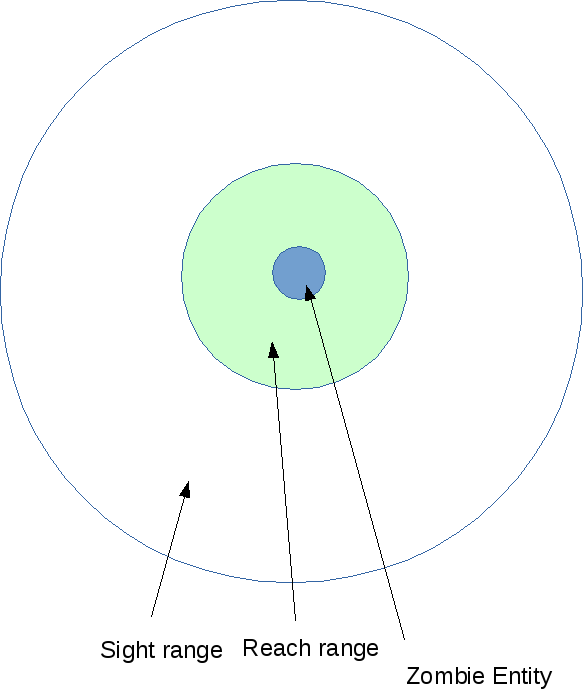
\includegraphics[width=0.3\textwidth]{img/zombie_range.png}
\caption{Illustration of a zombies sight and reach ranges}
    \label{fig:Illustration of a zombies sight and reach ranges}
\end{figure}
\subsubsection{Priorities}
The zombies priorities are very simple.Zombies prioritise killing humans above all else, if a human is within reach of the zombie it will try and kill and eat the human.The next priority is not being too close to another zombie, if another zombie is within reach then the zombies will attempt to move away from each other to prevent clustering together, this is to ensure that zombies form swarms rather than clustering together too closely and being unable to move away from each other due to getting surrounded by other entities.Next if a human is within sight of a zombie then the zombie will attempt to chase after the human, this allows zombies to break from swarming and attempt to kill humans.The next priority is forming a swarm with other zombies, this allows the zombies to form groups and combined with the previous priority will cause whole swarms of zombies to chase after humans even if not all of them can see the human. Finally if there is no other entities to interact with the zombies will move in an attempt to locate something to interact with.
\begin{figure}[h]
  \centering
  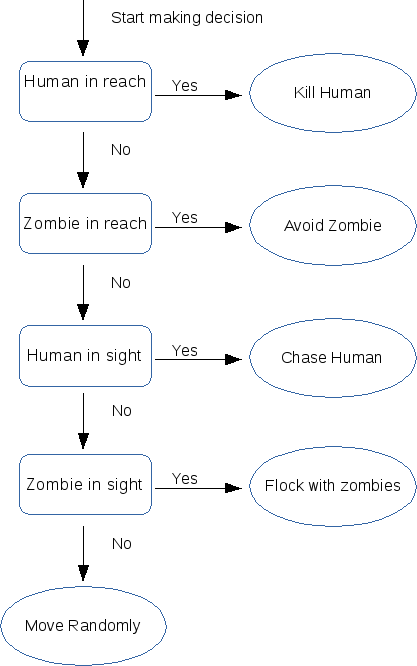
\includegraphics[width=0.3\textwidth]{img/zombie_decision_tree.png}
\caption{Zombie priorities diagram}
    \label{fig:Zombie priorities diagram}
\end{figure}
\subsubsection{Visibility}
To find all the humans and zombies within sight the zombie queries their viewer to receive lists of the human and zombie entities that the viewer is aware of, the zombie then iterates through these lists, calculating the distance of each entity from the zombie and removing any that are out of sight range.The zombie then cuts the list again to remove all entities that would be blocked from line of sight by obstructions.Finally the zombie sorts the list in order of distance so that the closest entities are first.
The zombie can then use these lists to determine it's action.
\subsubsection{Human entity within reach}
The highest priority is if a human entity is within reach of a zombie.if this happens the zombie will attempt to kill the human.There is a random chance the zombie will fail to kill the human, in which case it will just continue at the same velocity and nothing else happens this action. If the zombie succeeds it will still carry on at the same velocity but it will also pass a message to the human. This message will cause the human process to perform a function which creates a zombie entity in the humans location and kills the human entity.

\subsubsection{Zombie entity within reach}
The second highest priority is if there is another zombie within reach.If this is the case the acting zombie will attempt to avoid collision with the second zombie.This is based off the collision avoidance used in boids algorithms and is intended to stop a swarm of zombies from all clustering into a single point.The acting zombie will change its velocity to attempt to move in the opposite direction of the second zombie's location compared to the acting zombies. ie. if a second zombie is to the upper left of the acting zombie, the acting zombie will change velocity down and right.

\subsubsection{Human Entity within sight}
The third highest priority is if there is at least one human entity not within reach but within sight.The zombie will choose the closest human entity to it and change velocity in its direction. ie if there is a human five spaces above the zombie and another ten to the right, the zombie will change velocity up.

\subsubsection{Zombie entity within sight}
The fourth highest priority action is if there are zombie entities within sight but not reach, and there are no human entities within sight.The zombie will have two factors effecting its change in velocity in this case. Firstly the zombie will try to move towards the centre point of all zombies it can see, it does this by iterating through the list of zombie entities and averaging out their X and Y positions to find a target X and Y co-ordinate.It then calculates the direction and distance away the target is from its current position and changes its velocity by a fraction of those X and Y values.
Secondly the zombie will attempt to match the velocities of the other zombies it can see, this is calculated in the same way as moving towards the centre point, but uses the X and Y velocity of the other zombies instead.
the two resulting changes in velocity are added together to get the total change in X and Y velocity.
This action is also based off the boids algorithm, in particular the idea of flock cohesion and alignment.
\subsubsection{No entities in sight}
The lowest priority action is if there are no humans or zombies in sight.The zombie will start to change it's velocity randomly, this is to ensure that if a zombie has no targets it will still move and appear to search for other entities to interact with.

\subsection{Behaviour After Decision Making}
After making a decision the change in velocity resulting is added to the zombies current velocity then several limits will be checked to prevent the zombie moving against the rules of the simulation.

\subsubsection{Limit speed}
Zombies have a maximum distance they can move in one action,if the velocity of the zombie exceeds this value then a new velocity is calculated that keeps the same heading but with a distance at the maximum allowed, this prevents zombies moving unrealistically fast if they repeatedly change velocity to go the same direction.

\subsubsection{Energy}
Energy represents how recently a zombie has eaten. Energy decreases every time a zombie makes an action. If the energy of a zombie falls too low then the maximum distance a zombie can move per action is decreased to represent the zombie slowing down from hunger.Energy is refilled by killing humans and eating them.


\subsubsection{Obstructions}
If the spot the zombie intends to move to is obstructed either by another entity or an obstacle then the zombie will bounce off it to avoid collisions.If the obstacle is a wall, the zombie is placed next to the wall and its velocity is changed to -1 of whatever direction it hit the wall in but kept the same in the other axis to enable the zombie to keep moving without repeatedly hitting the wall again. If the zombie hit another entity it is placed next to the entity it hit but its velocity is not reset as there is little risk of repeatedly running into the same entity as all other entities will be moving at the same time.

\clearpage
\endinput
